\documentclass[12pt, oneside]{book}
\usepackage[a4paper,top=2.5cm,bottom=2.5cm,left=3.5cm,right=2cm]{geometry}
\usepackage[utf8]{inputenc}
\usepackage[T1]{fontenc}
\usepackage{graphicx}
\usepackage{url}
\usepackage[english]{babel} % vypnite pre prace v anglictine
\usepackage{color}
\usepackage{stmaryrd}
\usepackage{amsmath} 
\usepackage{amsthm}
\usepackage{listings}
\usepackage{caption}
\usepackage{subcaption}
\usepackage{float}
\usepackage[final]{pdfpages}
\usepackage[none]{hyphenat}
\usepackage{algorithm2e}


\lstset{
        mathescape=true,
        literate=
               {=}{$\leftarrow{}$}{1}
               {==}{$={}$}{1},
        morekeywords={if,then,else,return,for,def}
        }


\theoremstyle{definition}
\newtheorem{definition}{Definition}[section]


\linespread{1.25} % hodnota 1.25 by mala zodpovedat 1.5 riadkovaniu

% -------------------
% --- Definicia zakladnych pojmov
% --- Vyplnte podla vasho zadania
% -------------------
\def\mfrok{2018}
\def\mfnazov{Improving LSA word weights for document classification}
\def\mftyp{Diploma thesis}
\def\mfautor{Bc. Vladimír Macko}
\def\mfskolitel{RNDr. Kristína Malinovská, PhD.}
\def\*{{\color{red} \bf FIXME: }}

%ak mate konzultanta, odkomentujte aj jeho meno na titulnom liste
\def\mfkonzultant{RNDr. Radim Řehůřek, PhD.}  

\def\mfmiesto{Bratislava, \mfrok}

%aj cislo odboru je povinne a je podla studijneho odboru autora prace
\def\mfodbor{ 2508 Computer Science } 
\def\program{ Computer Science }
\def\mfpracovisko{ Department of Computer Science }

\begin{document}     

% -------------------
% --- Obalka ------
% -------------------
\thispagestyle{empty}

\begin{center}
\sc\large
COMENIUS UNIVERSITY, BRATISLAVA\\
FACULTY OF MATHEMATICS, PHYSICS AND INFORMATICS

\vfill

{\LARGE\mfnazov}\\
\mftyp
\end{center}

\vfill

{\sc\large 
\noindent \mfrok\\
\mfautor
}

\eject % EOP i
% --- koniec obalky ----

% -------------------
% --- Titulný list
% -------------------

\thispagestyle{empty}
\noindent

\begin{center}
\sc  
\large
COMENIUS UNIVERSITY, BRATISLAVA\\
FACULTY OF MATHEMATICS, PHYSICS AND INFORMATICS

\vfill

{\LARGE\mfnazov}\\
\mftyp
\end{center}

\vfill

\noindent
\begin{tabular}{ll}
Study Program: & \program \\
Branch of Study: & \mfodbor \\
Department: & \mfpracovisko \\
Supervisor: & \mfskolitel \\
Advisor: & \mfkonzultant \\
\end{tabular}

\vfill


\noindent \mfmiesto\\
\mfautor

\eject % EOP i


% --- Koniec titulnej strany


% -------------------
% --- Zadanie z AIS
% -------------------
% v tlačenej verzii s podpismi zainteresovaných osôb.
% v elektronickej verzii sa zverejňuje zadanie bez podpisov

\newpage 
\thispagestyle{empty}
%TODO
%\hspace{-2cm}\includegraphics[width=1.1\textwidth]{images/zadanie}
%\includepdf[pages={1}]{/home/maja/Documents/matfyz/diplomovka/text/zadanie.pdf}

% --- Koniec zadania

\frontmatter

% -------------------
%   Poďakovanie - nepovinné
% -------------------
\setcounter{page}{3}
\newpage 
~

\vfill
{\bf Acknowledgment:} \*

% --- Koniec poďakovania


% -------------------
% --- Abstrakt - Anglicky 
% -------------------
\newpage 
\section*{Abstract}
\*

\paragraph*{Keywords:} natural language processing, document classification, LSA, gradient descent

% --- Koniec Abstrakt - Anglicky


% -------------------
%   Abstrakt - Slovensky
% -------------------
\newpage 
\section*{Abstrakt}
\*

\paragraph*{Kľúčové slová:} spracovanie prirodzeného jazyka, klasifikácia dokumentov, LSA, gradient descent
% --- Koniec Abstrakt - Slovensky


% -------------------
% --- Predhovor - v informatike sa zvacsa nepouziva
% -------------------
%\newpage 
%\thispagestyle{empty}
%
%\huge{Predhovor}
%\normalsize
%\newline
%Predhovor je všeobecná informácia o práci, obsahuje hlavnú charakteristiku práce 
%a okolnosti jej vzniku. Autor zdôvodní výber témy, stručne informuje o cieľoch 
%a význame práce, spomenie domáci a zahraničný kontext, komu je práca určená, 
%použité metódy, stav poznania; autor stručne charakterizuje svoj prístup a svoje 
%hľadisko. 
%
% --- Koniec Predhovor


% -------------------
% --- Obsah
% -------------------

\newpage 

\tableofcontents

% ---  Koniec Obsahu

% -------------------
% --- Zoznamy tabuliek, obrázkov - nepovinne
% -------------------

%\newpage 

%\listoffigures

% ---  Koniec Zoznamov

\mainmatter

\input text.tex 


\input conclusion.tex

% -------------------
% --- Bibliografia
% -------------------


\newpage	

\backmatter

\thispagestyle{empty}
\nocite{*}
\clearpage

\bibliographystyle{plain}
\bibliography{literatura} 


%---koniec Referencii

% -------------------
%--- Prilohy---
% -------------------

%Nepovinná časť prílohy obsahuje materiály, ktoré neboli zaradené priamo  do textu. Každá príloha sa začína na novej strane.
%Zoznam príloh je súčasťou obsahu.
%
\addcontentsline{toc}{chapter}{Appendix A}
\input AppendixA.tex
%
%\addcontentsline{toc}{chapter}{Appendix B}
%\input AppendixB.tex

\end{document}






